\section{Literature Review}

\subsection{Prior Work in Subject Area}
Stefan et al.\ found that \enquote*{the intention not to waste food does not have a
significant effect on reported food waste}. Instead, planning before shopping to
check what is already available was found to lead to a reduction in food waste.~\cite{stefan_avoiding_2013}

As planning before shopping is a key factor in reducing food waste, the need for a system
that tracks how much of each ingredient is available was identified. This would allow for
users to know plan meals based on what they already have, reducing the need to buy more ingredients
and thus reducing food waste.

\label{sec:overload_intro}While providing a user with variety of choices can improve their satisfaction
with the overall system, care must be taken to avoid information overload.
Bollen et al.\ found that offering a more limited set items predicted to be among a user's
highest rated, followed by a larger set of more varied items with lower rankings, led to
higher satisfaction on average.~\cite{bollen_understanding_2010}

Currently, the app shows all suggestions at once, but with further development, this could be
reduced to a more limited subset of the suggestions, with the option to view more if desired and is
discussed in further detail in Section~\ref{sec:choice_overload}.

The motivation for the \chef{} app is two-fold: to reduce the environmental impact of food waste and to
save costs for households by allowing them to collectively track what ingredients are available to them.

\subsubsection{Techniques Common to Food Reccomendation Systems}
There exist a broad range of techniques used by food recommendation systems, using both machine learning
and statistical models, the most popular method in existing studies being machine learning based on the
contents of recipes. Most of which were not personalized to the individual user.~\cite{bondevik_systematic_2024}

Among prior systems, the majority source their training data from textual data with the most commonly used
attributes being ingredients, cooking instructions, and the recipe title itself. There has been limited research
into combining multiple attributes of the recipe or giving attributes different weights.~\cite{chen_cross-modal_2017} These factors are often
considered to be merely a subject for future research or unimportant, which is believed to degrade the performance
of systems.~\cite{bondevik_systematic_2024}

\subsection{Recipe Name-based Suggestions}
\todo{Recipe Name-based Suggestions}

\subsubsection{Effectiveness Outside of Western Cuisine}
While western recipe names are typically constructed in a predictable format
that indicates what kind of recipe it is, this is not the case world-wide.
For example, Chinese recipe names often bear little resemblance to the contents
of the recipe itself.~\cite{wang_substructure_2008} This limits the effectiveness
of suggestions systems based on names and as such a more complex system as discussed
by Wang et al.\ would be needed.
\todo{ai recipe suggestion}

\subsection{Gaps in Existing Literature}
\todo{Gaps in existing literature}

\subsection{Recipe Datasets}
\todo{Recipe Datasets}

\subsection{The Research Question}
\todo{The Research Question. This is covering what the app is doing and how the goal is a robust app that does the job.}

The goals of the \chef{} app is to provide a robust system that allows for users to track what ingredients they have in a
convenient manner, and to suggest recipes based on these ingredients, user preferences, dietary requirements, and to find
similar recipes that meet these criteria.

\todoinline{
    A literature review has four main objectives:
    • Outlines the area you are researching --- what is the context of your work?

    • Explain why it matters --- what is the state of the art in your project area?

    • Summarises prior research that has been done in this area, particularly any key studies

    • Identifies any gaps in the literature to justify why your study is important and what it adds to the literature

    • Identifies a set of possible techniques/methods for solving the problem

    • Presents your research questions as the natural conclusion of the literature review (this is especially relevant for investigative projects)

    A literature review is *not* just a summary! It provides a firm foundation for your project work

    Identify and synthesize the existing papers on the topic

    2500--3000 words

    Organize papers while reading and make notes on them. Could include these notes as an appendix

    See the blackboard tool to evaluate how good the paper is (week 4 lecture)

    Can review software, but should be primarily academic work. Could also have a different section for software

    can still download the original file.

    How to structure the lit review chapter
        • Give it a structure
        • introduction giving scope
        • body with sections (see next slide)
    • conclusions
    • Identify themes
    • Give a succinct, careful account of each theme after assimilating all the ideas from the material
    • Discuss the work reviewed and give your perspective
    • Draw out conclusions and applications to your project

    How to structure the body of a lit review
    Consider three common structures:
    • Chronological: you write about related work according to when each paper was published.
    • Thematic: Thematic reviews of literature are organized around a topic or issue, rather than the progression of time. However,
    the progression of time may still be an important factor in a thematic review.
    • Methodological: A methodological approach differs from the two above in that the focusing factor usually does not have to do with the content of the material.
    Instead, it focuses on the “methods” of the researcher or writer. Use PEE structure (Point, Evidence, Explain) for each paragraph

    Other elements of a lit review chapter• Use evidence: A literature review must be backed up with evidence to show that what you are saying is valid.
    • Be selective: Select only the most important points in each source to highlight in the review. The type of information you choose to mention should relate
    directly to the review's focus, whether it is thematic, methodological, or chronological.
    • Use quotes sparingly: Some short quotes here and there are okay, though, if you want to emphasize a point, or if what the author said just cannot be rewritten in your own words.
    For example, you can quote certain terms that were coined by the author, not common knowledge, or taken directly from the study.
    • Summarize and synthesize: Remember to summarize and synthesize your sources within
    each paragraph as well as throughout the review.
    • Keep your voice: While the literature review presents others' ideas, your voice (the writer's) should remain front and centre.
    For example, weave references to other sources into your text, but you can still maintain your voice by starting and ending the paragraph with your ideas and
    your own words. The sources then act as a way of supporting what you are saying.• Use caution when paraphrasing: When paraphrasing a source that is not your own, be sure to
    represent the author's information or opinions accurately and in your own words. You still need to reference the source to avoid plagiarism.

    A literature review is not:
    • Describing very basic material etc.
    • Things you can assume your reader knows.
    • Justifying your choice of project topic
    • Normally, the introduction should cover this
    • Extensive history of computing / the Internet etc.
    • May wish to cover the development of ideas in your field, briefly, but consider relevance.
    • Write down everything you have learned.
    • All of these will suggest a weak project report

    Assume the reader has a basic knowledge of computing. Don't overuse jargon

    Common issues with lit reviews
    • Simply list each book/paper you have read with a summary of it
    • Quoting or closely paraphrasing long passages
    • Trying to cover many topics and give very little on each.
    • Find one source on each topic and stop there. You cannot build an argument around consensus \enquote*{literature states} with one source.
    • You can dismiss other approaches --- while demonstrating you are aware of them, e.g., \enquote*{I refer to [key term] as described by Creswell and Creswell (2018). For other common uses see Y (2014), and Z and X (2015)}.
    • No attempt at critical engagement of the literature provided. Not all literature is created equal or is equally as useful to you.
    • There is literature, but it lacks an argument. It's there, but not in support of any central argument.
    • Not using the literature to its full advantage. Pick key figures out of quotes:
    \enquote*{Smith (2011) agrees there is a large increase in figures in this area} OR
    \enquote*{Smith (2011) highlights the significance of the increase in the sector, asserting there was a 57\% increase within 5 years from 2012--2017}
    • No literature at all!

    Look at the academic phrase bank
}

\section{Competitor Analysis}\label{sec:competitor_analysis}
\todo{Need more here. Discuss the positives and negatives of each competitor.}

As part of the development of \chef{}, a competitor analysis has been performed on several existing solutions as part of research
into the problem domain. These solutions, while useful, had limitations as discussed below. The \chef{} app aims to address
these limitations and provide a more useful solution. The full list of competitors analysed is provided in Section~\ref{sec:competitors}.

SuperCook and MyFridgeFood both include feature an account system
that saves a user's list of available ingredients. Creating an account also allows for recipes to be favourited/bookmarked
which would then be shown on a dedicated page. SuperCook additionally shows which of the user's favourite recipes
can be made using available ingredients and which ingredients are missing. Both apps also use exclusively imperial
units for ingredients that are not understood by the majority of the world. The \chef{} app will use metric units by default
as it is targeted at a UK audience.

However, neither of these apps has a system for sharing pantries between users or specifying disliked ingredients. These features would be useful for households with multiple people.
Additionally, the only way to update available ingredients is to manually add or remove them which is time-consuming and tedious. There is no tracking for the quantity of
each ingredient, so there is no way to know if the user has enough of an ingredient without checking manually.

Neither app tracks which recipes have been made recently, so there is no way to avoid suggesting similar recipes to ones that have been recently made which could lead to
users getting bored with eating the same meals over and over.

MyFridgeFood has a feature to submit new recipes which are shared between all users. This is a useful feature as it allows for the community to contribute to the database
of recipes, however, these cannot be kept private to just one user.

\subsection{User Reviews}

A frequent complaint about MyFridgeFood was that it suggested
recipes that users lacked ingredients for. See figure~\ref{rev:review_missing_ingredients} for an example.

Another user found that MyFridgeFood gave them suggestions that were too similar to each
other. See figure~\ref{rev:review_lack_variety} for the review.

\section{Product Requirements}

\todo{Where did these specificvations come from? How did you develop them?}

% https://tex.stackexchange.com/questions/503668/increment-a-counter
\newcounter{functionalreqcounter}
\newcommand{\requirementtype}{FR}
% Usage:
%   #1 Requirement
%   #2 Source
%   #3 Priority
%   #4 Implemented (yes/no)
\newcommand{\requirement}[4]{%
    \requirementtype\stepcounter{functionalreqcounter}\arabic{functionalreqcounter}%
    % Don't have much space to work with, so flushright looks messy.
    &\raggedright#1&#2&#3&#4\\}

\begin{longtable}{lp{128pt}lll}
    \caption{Functional Requirements}\label{tab:functional_requirements}
    \\\toprule
    \textbf{ID} & \textbf{Requirement} & \textbf{Source} & \textbf{Priority} & \textbf{Implemented} \\\midrule

    \requirement{\label{req:web_app}\newcounter{webappid}\setcounter{webappid}{\thefunctionalreqcounter}%
        \textbf{Web app.} The system \textbf{must} be a web app that fetches from a REST API}
    {Competitor Analysis}
    {Must-have}
    {Yes}

    \requirement{\textbf{User registration.} The system \textbf{must} allow users to sign up and log in to the app.}
    {Competitor Analysis}
    {Must-have}
    {Yes}

    \requirement{\textbf{Share ingredient lists.} The system \textbf{must} allow for multiple users to share one \virtualfridge{}}
    {Competitor Analysis}
    {Must-have}
    {Partially}

    \requirement{\textbf{Select dietary requirements/preferences.} The system \textbf{must} \newline
        allow for users to select their dietary requirements and preferences, such as allergies or disliked ingredients.}
    {Competitor Analysis}
    {Must-have}
    {Yes}

    \requirement{\textbf{Recipe Suggestion.} The system \textbf{must} suggest recipes based on the user's available ingredients}
    {Competitor Analysis}
    {Must-have}
    {Yes}

    \requirement{\textbf{Avoid recipes with missing ingredients.} The system \textbf{must} not suggest recipes that the user
    is missing ingredients for unless explicitly requested.}
    {Competitor Analysis}
    {Must-have}
    {Yes}

    \requirement{\label{req:sources}\newcounter{sourcesid}\setcounter{sourcesid}{\thefunctionalreqcounter}%
    \textbf{Include sources.} The system \textbf{must} include its sources for recipes.}
    {Trivial}
    {Must-have}
    {Yes}

    \requirement{\label{req:data_flexible}\newcounter{flexibleid}\setcounter{flexibleid}{\thefunctionalreqcounter}%
    \textbf{Flexible Data Sources.} The system \textbf{should} be flexible regarding the dataset it uses}
    {Dataset Selection}
    {Should-have}
    {Yes}

    \requirement{\textbf{Scan barcodes.} The system \textbf{should} allow the user to scan the barcodes of ingredients to add
    them to their \virtualfridge}
    {Use Case Analysis}
    {Should-have}
    {Yes}

    \requirement{\label{req:track_amounts}\newcounter{trackamountsid}\setcounter{trackamountsid}{\thefunctionalreqcounter}%
    \textbf{Track ingredient amounts.} The system \textbf{should} track the amount of each ingredient the user has available.}
    {Competitor Analysis}
    {Should-have}
    {Yes}

    \requirement{\textbf{Use metric units.} All units \textbf{should} be displayed in metric by default.}
    {Competitor Analysis}
    {Should-have}
    {Yes}

    \requirement{\textbf{Optionally use imperial units.} There \textbf{could} be an option to display imperial units instead of metric.}
    {Competitor Analysis}
    {Could-have}
    {No}

    \requirement{\textbf{Scan receipt.} The system \textbf{could} allow the user to scan a receipt from a store to add ingredients
    to their \virtualfridge}
    {Use Case Analysis}
    {Could-have}
    {No}

    \requirement{\label{req:similar_recipes}\newcounter{findsimilarid}\setcounter{findsimilarid}{\thefunctionalreqcounter}%
    \textbf{Find similar recipes.} The system \textbf{should} use a machine learning model to find and suggest
    similar recipes to those that the user has previously made.}
    {Literature Review}
    {Should-have}
    {Yes}

    \requirement{\label{req:too_similar}\newcounter{toosimilarid}\setcounter{toosimilarid}{\thefunctionalreqcounter}%
    \textbf{Avoid repeating recipes.} The system \textbf{should} avoid suggesting recipes that are too similar
    to those that have been made recently using the same model as \hyperref[req:similar_recipes]{FR\arabic{findsimilarid}}}
    {Competitor Analysis}
    {Should-have}
    {No}

    \requirement{\textbf{Single sign on.} The system \textbf{won't currently} support single sign on.}
    {Competitor Analysis}
    {Won't-have}
    {No}

    \requirement{\textbf{Add recipes.} The system \textbf{won't currently} allow for users to add their own recipes to the database.}
    {Competitor Analysis}
    {Won't-have}
    {No}

    \bottomrule
\end{longtable}

\setcounter{functionalreqcounter}{0}\renewcommand{\requirementtype}{NFR}
\begin{longtable}{lp{128pt}lll}
    \caption{Non-functional Requirements}\label{tab:non_functional_requirements}
    \\\toprule
    \textbf{ID} & \textbf{Requirement} & \textbf{Source} & \textbf{Priority} & \textbf{Implemented} \\\midrule

    \requirement{\textbf{Performance.} The system \textbf{should} be responsive to user input and requests to the API \textbf{should}
    be responded to in under 200ms on average.}
    {Trivial}
    {Should-have}
    {Yes}

    \requirement{\textbf{Reliability.} The system \textbf{should} be reliable and resilient should the user incorrectly use an element of
    the app.}
    {Trivial}
    {Should-have}
    {Yes}

    \requirement{\textbf{Usability.} The system \textbf{should} be intuitive and easy to use.}
    {Trivial}
    {Should-have}
    {Yes}

    \requirement{\textbf{Maintainability.} The system \textbf{should} be structured in a way that is maintainable and upgradable
    in the future.}
    {Trivial}
    {Should-have}
    {Yes}

    \requirement{\textbf{Code quality.} The system \textbf{must} pass all of its unit tests.}
    {Trivial}
    {Must-have}
    {Yes}

    \requirement{\textbf{Ease of setup.} The system \textbf{should} be installable using a single script and minimal manual input.}
    {Trivial}
    {Should-have}
    {Yes}

    \requirement{\label{req:localization}\newcounter{localizationid}\setcounter{localizationid}{\thefunctionalreqcounter}%
        \textbf{Localization.} The system \textbf{won't currently} support multiple languages.}
    {Trivial}
    {Won't-have}
    {No}
    \bottomrule
\end{longtable}

\subsection{Sequence Diagrams}

Before designing the user interface, use case diagrams were created to show the flow of the system. These are included in Section \ref{sec:sequence_diagrams}
of the appendix.

\todoinline{
    Summarize the requirements for the product to be built.

    How will you/did you:
    • Discover, specify, prioritise, justify them?
    • Do they come from clients? Literature? Competitors? Your head? Somewhere else?
    • Your requirements specification is counted as part of the Product
    • The spec and the report chapter are not the same thing!
    • A DISCUSSION AND JUSTIFICATION of the requirements is expected in the report

    Functional requirements --- what the system does.
    • Processing, inputs, outputs, data\ldots
    • Non-functional requirements --- how it does it.
    • Software quality: performance, throughput, availability etc.
    • Usability \& user characteristics
    • Environment --- physical, organisational etc.
    • Required computing hardware, software tools etc

    Use MoSCoW requirements, W stands for would like to have, but won't currently

    Someone should be able to build the product based only on the list of requirements

    One option for structuring your requirements document is to follow the IEEE template.

    • ISO/IEC/IEEE 29148

    http://ieeexplore.ieee.org/xpl/mostRecentIssue.jsp?punumber=6146377

    • IEEE 830--1998 (older)

    http://ieeexplore.ieee.org/xpl/articleDetails.jsp?arnumber=720574

    • You don't have to use this --- but
        • it gives you a structure that you can adapt
        • it can encompass various approaches such as use case modelling.
        • Other templates available.
}

\section{Approach/Methodology}

This study is primarily into the algorithm used to suggest recipes. For this reason,
it was decided not to perform interviews or user testing. Instead, unit tests will
be the primary testing method.

\todo{Approach/Methodology}

\todo{Should go into each of the requirements, justify them, and discuss how they will be implemented}

\subsection{Choice of Language (FR\arabic{webappid})}\label{sec:language}

There are numerous languages and frameworks that can be used to build a web application including
Django (Python), Laravel (PHP), ASP.NET (C\#), and React (JavaScript/TypeScript), each of which has
its strengths and weaknesses.

Django is a Python web framework designed to include all the features needed for a web application such
as an ORM, authentication, and localization (which would have made NFR\arabic{localizationid}
easier to implement).~\cite{ghimire_comparative_2020} Additionally, Python is considered to be an
industry standard for machine learning tasks. However, it is considered to be a slow language\cite{srinath_pythonfastest_2017}
which, coupled with a lack of personal experience beyond simple scripts, made it an unattractive choice.

Laravel is a PHP web framework that functions similarly to Express, with routes being defined as a series of
middleware functions called when a request is made. User-facing pages are built using the Blade templating engine
which combines HTML with PHP in a neater syntax than standard PHP.~\cite{nguyen_building_2015,he_design_2015}
However, there were concerns about the suitability of PHP for machine learning tasks which would be needed for
\hyperref[req:similar_recipes]{FR\arabic{findsimilarid}}.

ASP.NET is a web framework based on the DotNet platform, which is primarily used with the C\# language.
Similar to Django, it supports templated views in a syntax that combines HTML with C\# code. The C\# language
itself uses a very similar syntax to Java and supports features such as nullable types and pattern matching
which can help to prevent bugs.~\cite{gao_type_2017} An external library, TorchSharp, can be used to run
PyTorch models in C\# which could serve as the backend for machine learning integration. However, despite
a familiarity with C\# from previous projects, the lack of experience with ASP.NET made it a less attractive
choice.

React is a JavaScript-based frontend library that is used to build user interfaces with a component-based,
HTML-like syntax. It features an event-driven architecture where components only update when their state changes,
such as in response to user input or an API request completing. This is efficient as it minimizes data transfer
between the client and server and only re-renders components that have changed.

Unlike the other frameworks considered, which run server-side, React is purely a client-side library and thus
needs to communicate with a backend server in order to fetch data. While React can fetch from any server-side
library, Express.js running on Node.js allows for both components to be written in the same language, simplifying
the development process by allowing code and library reuse.

Both React and Node are based on JavaScript, which is a dynamically typed language and thus gives no guarantees
as to the type of data that is being passed around the system. Instead, TypeScript can be used and compiled to
JavaScript to add static type checking to the system. This can prevent many bugs from being introduced that would
otherwise not be detected until later, especially with the checks for \texttt{null} and \texttt{undefined} enabled.~\cite{gao_type_2017}
For this reason, TypeScript was the language of choice for both React and Node. See Figure \ref{fig:type_check} for an
example of some issues that TypeScript can catch pre-emptively that JavaScript cannot.

\subsection{The Dataset (FR\arabic{sourcesid}, FR\arabic{flexibleid}, FR\arabic{trackamountsid})}\label{sec:data_pre_process}

It was decided to use a pre-existing dataset for the app in order to save time by removing the need to manually enter recipes
or create a web scraper to gather them, and is both a legal and ethical grey area.~\cite{murray_state_university_legality_2020}

The Recipe Box~\cite{lee_recipe_2017} dataset was initially considered, but later disregarded as the pre-scraped download only includes the
hashed versions of the source URLs and the scraping scripts no longer function due to changes in website design. This would have made
\hyperref[req:sources]{FR\arabic{sourcesid}} impossible to achieve.

An additional dataset that was considered was the Food.com Recipes and Interactions dataset~\cite{li_foodcom_2019}. However, this only includes
ingredient names and not amounts, which was insufficient to cover \hyperref[req:track_amounts]{FR\arabic{trackamountsid}}

In the end, RecipeNLG~\cite{bien_recipenlg_2020} was the dataset of choice for the \chef{} app. This contains approximately 2 million recipes
each with an ingredient list, a list of directions, and its source URL. This dataset was chosen as it includes all the features needed to
fulfill the requirements of the app and is available freely for research and educational purposes.

If the app proved to be successful, a different or custom dataset could be used as the app is designed
to be flexible in this regard, as the setup script is the only component to interact with the dataset. (FR\arabic{flexibleid})

See table~\ref{tab:recipenlg_row_format} for the information that is included with each recipe and that is imported into
the app's database during setup. The schema script for the database is located at \texttt{./app/backend/data/schema.sql}
in the project's Git repository and is not included in this report due to its length.

\begin{table}[h]
    \caption{RecipeNLG Row Format}\label{tab:recipenlg_row_format}

    \begin{tabulary}{\textwidth}{llL}
        \toprule
        \textbf{Name} & \textbf{Type} & \textbf{Description} \\\midrule

        Title & String & The name of the recipe.\\

        Ingredients & String array & A list of ingredients along with the quantity required. Quantities are presented in imperial units.\\

        Directions & String array & A list of directions to make the recipe. Temperatures are presented in Fahrenheit.\\

        Link & String & A link to the page where the recipe was sourced.\\

        Source & String & The dataset the recipe was sourced from, \enquote*{Gathered} for recipes collected for RecipeNLG itself or the name of another dataset.\\

        NER & String array & A list of ingredients without quantities.\\
        \bottomrule
    \end{tabulary}
\end{table}

\begin{table}[h]
    \caption{\label{tab:sample_entry}A sample entry from RecipeNLG}
    \begin{tabulary}{\textwidth}{lL}
        \toprule
        \textbf{Column}&\textbf{Value}\\\midrule
            Title & No-Bake Nut Cookies\\
            Ingredients & [\enquote*{1 c.\@ firmly packed brown sugar}, \enquote*{1/2 tsp.\@ vanilla}, \ldots]\\
            Directions & [\enquote*{In a heavy 2-quart saucepan, mix brown sugar, nuts, evaporated milk and butter or margarine.},
            \enquote*{Stir over medium heat until mixture bubbles all over top.}, \ldots]\\
            Link & \href{www.cookbooks.com/Recipe-Details.aspx?id=44874}{www.cookbooks.com/Recipe-Details.aspx?id=44874}\\
            Source & Gathered\\
            NER & [\enquote*{brown sugar}, \enquote*{milk}, \ldots]\\
        \bottomrule
    \end{tabulary}
\end{table}

\subsubsection{Data Pre-processing}
Many existing papers in the area do not pre-process their recipe data. Among those that do, the most
common methods are text cleaning and exclusion, with duplicate removal being a rare step to undertake.~\cite{bondevik_systematic_2024}

Duplicate removal was deemed the only pre-processing necessary for the \chef{} app due to similarity being
based on the recipe name (see Section~\ref{sec:recipe_similarity}). Therefore, any number of recipes with the same
name would be considered identical. Instead, the import script discards any recipe with a name that has been seen before.

The dataset used contains a number of meaningless and nonsensical recipes (see
figure~\ref{fig:bad_recipe_entry}), which were imported by the \chef{} system during setup.
A possible reason for these being included in RecipeNLG is that some
data sources scraped for it allow for user-submitted recipes, this contributes to
an unclean and noisy dataset.~\cite{kicherer_what_2018}

\begin{figure}[p]
    \centering
    \caption{\label{fig:bad_recipe_entry}A nonsensical recipe that was included in the dataset.}
    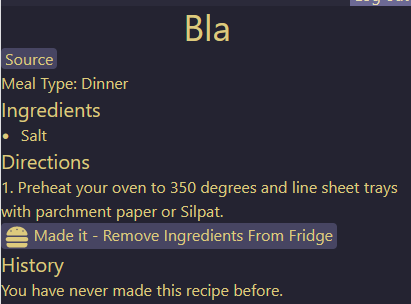
\includegraphics[scale=0.75]{figures/bad_recipe_entry.png}
\end{figure}

A possible solution for this issue would have been to further pre-process the data beyond what is
discussed in Section~\ref{sec:data_pre_process} to remove or correct noisy entries that would otherwise
harm the quality of the system.~\cite{garcia_big_2016} This was not considered a priority due to time
constraints and the fact that the noise had minimal impact on the system's results.

\subsection{Recipe Similarity Algorithms (FR\arabic{findsimilarid})}\label{sec:recipe_similarity}
\todo{Recipe Similarity Evaluation}
The similarity of recipes can be evaluated using a sentence embedding model \todo{Source}.

For the \chef{} app, the pre-trained Universal Sentence Encoder~\cite{cer_universal_2018} was decided upon.
This can run in a Node.js environment via TensorFlow.js.

The cosine similarity metric, as used in the original USE paper, can be used to evaluate the similarity of
embeddings as a score normalized between 0 and 1. This metric provides higher precision and
recall than other metrics which make it an effective measure for ranked retrieval from
queries.~\cite{ihajeer_comparison_2012}
\todo{https://ieeexplore.ieee.org/abstract/document/7032612}

\section{Commentary on Requirements Specification}
\todo{Commentary on Requirements Specification. Discuss the specification, which is a separate document}

\todoinline{
    Research and Planning
    The research and planning section may consist of several chapters. The exact number will depend upon the nature of the work you are undertaking.
    Typically, this part of the report should provide the reader with information they will need to know to appreciate and understand the work you have done in
    the rest of the project. You should assume a computer-literate reader but not a specialist in your particular topic.
    The research and planning follow from the background given in the introduction. The marking scheme asks for the following five areas to be covered:
    •	Clear identification and analysis of the problem to be looked at, identifying the key technical or other problems to be solved. Necessary background material
    that goes beyond the scope of the introduction may be included.
    •	A critical review of literature related to the topic; this will normally address some combination of the underlying principles of the problem area and
    possible approaches to solving the problem. The relevance of these ideas to the project should be clear.
    •	Discussion of approaches appropriate for the solution of the problem.
    •	A discussion and justification of the product requirements if a product will be built.
    •	Explanation and justification of the tools and techniques to be used in the project work.

    Note that while all these elements are suggested, they do not necessarily map onto five separate chapters of your report. For example, a discussion of approaches to
    solving the problem may fit naturally after your literature review. “Tools and techniques” here refer to what you use to build the product or conduct
    the investigation, while “approaches” is used to include higher-level issues such as an overall strategy or architecture, the choice of implementing one algorithm rather
    than another to carry out a task, a general type of solution, etc. You should arrange the material in chapters in whatever way that best suits your project. Some projects
    will not even require all five areas. Ensure that you include everything necessary for your project.

    Your research and planning should include a discussion of the wider issues, and critically examine the methods that might be used in solving the problem and any constraints
    that apply. Beware of presenting a shallow treatment of the subject which might be obtained from standard texts. You are expected to support your argument by exploring
    academic literature which is seminal and up-to-date.

    The background and problem description should describe the actual problem you are looking at and set it in context. You should tell the reader about the computing problems
    to be investigated, the product to be built, etc., as relevant, building on the brief overview given in the introduction. Bring out features of the problem you would not
    expect the reader to know about. Do not state the obvious.

    The literature review will be a very important component of the research. Your literature review may discuss the problem that you are trying to solve, the question that
    you are trying to answer, possible solutions, methods of investigation, etc., as appropriate to your needs. You need to find out the state of the art --- what others have
    done in this area, what solutions have been proposed, what findings have been achieved, what products have been created to tackle the same problem, and what
    tools/techniques/approaches have been proven to be useful. The purpose is to help you analyse the problem and its context, learn from existing related work, and
    propose appropriate solutions for your project. You need to look for important concepts and principles, possible techniques, methods, tools, structures, etc that
    you could use in your project.
    Note that the marking scheme says that a \enquote*{critical review} is required. You should not simply be relaying information or paraphrasing the sources that you have found, but
    identifying principles, structuring ideas, discussing the relevance to your project, and making evaluative comments about what you have found. It is useful to end the
    literature review by summarising the key ideas that it has contributed to the project.

    Another pitfall to avoid is attempting to write about too many areas. You may find that there is a great deal of relevant literature and many subjects to review. It is
    better to aim for depth in the areas that are necessary and relevant to your project. An opposite example is the review where many areas are tackled but nothing
    of significance is said about any of them, and perhaps only one source (or no sources!) is cited for each. In this case, assuming that the project topic is suitable, the
    student would have been better advised to take a narrower focus.

    The length of a literature review should be guided by the needs of the specific project, but they are typically 2500--3000 words. You should use respectable academic sources,
    such as refereed journals conferences, or other reliable and authoritative sources of information.

    Once you have described your problem and put it into context by carrying out the literature review, you are in a position to identify and justify the appropriate approach
    to take to solve the problem. You will need to explain your approach at an overview level and give your reasons for choosing this approach. We are looking for a
    high-level discussion here. You will go into the details of exactly what you did (e.g., how you built the product, set up experiments, chose your participants, ran your
    tests, etc.) in the practical work chapters.

    If your practical work is to investigate a research question/hypothesis, you should discuss the possible strategies for conducting research or
    investigations in your subject area. This could be quite different for projects in different subject areas, for example, forensics, networking or HCI.\@ You may need to
    consider research methods --- for example, are you using one of the many varieties of experimental design? are you carrying out your study in lab conditions or the
    field? will you be taking measurements of the performance of real equipment, or using a computer simulation? You should review the possible alternative approaches, and
    explain why your chosen strategy was preferable to others, or was the only possibility.

    If you plan to build a product, you need to identify the requirements for the product and produce its specifications. The actual specification of requirements is part
    of your product and is marked under the product component. The research and planning chapters include your discussion and justification of those requirements. Reasons
    for choosing particular requirements could relate to user needs, constraints on project scope, the findings of your literature review, etc., --- whatever is appropriate
    to your particular project. You should discuss the methods you used to establish the product requirements, e.g., requirements elicitation and modelling, interviews,
    and examination of existing products. It is appropriate to comment on significant findings that affect the decisions and to include any artefacts produced and the outputs
    of your investigations in the product documentation. It is expected that your requirements specification covers both functional and non-functional requirements. It is
    expected that your requirements specification covers both functional and non-functional requirements.

    You must also identify and justify the methods, tools, and techniques that you will use to conduct your investigation and/or build your product. Again, the decisions
    should be based on a literature review and/or examination of related work. You should justify that the chosen tools and methods are appropriate for solving the problem
    and meeting the requirements, and explain the deliverables that you are going to produce.
    You may find that you now have several possible approaches and technologies that could be used to solve the problem. If this is the case, you should provide a short
    analysis of the possibilities justifying your selected route if the factors influencing your choices are worth discussing. There is no point in going through a spurious
    decision process if there is no real decision to be made. Many students choose a programming language database or other software tool because they are familiar with it.
    As long as the tool is suitable, your familiarity with it is a sufficient reason for using that technology, and it is sufficient to indicate briefly why it is appropriate.
    If your project requires the use of some very specialised software or programming language, it may be useful to describe its main features as well as justify its use,
    and if the focus of your project is exploring a particular tool or tool features, you will, of course, need to discuss the features in some depth. It is also suggested
    to briefly discuss the alternatives if the chosen tools/techniques do not work as expected. For some projects, there will not be any realistic alternatives to the tools
    and techniques that you are using. This is not a problem as long as you can justify it.
}
